\chapter{Tecnología usada}

Una vez introducidos en el proyecto y con los objetivos marcados se hablara de las tecnologías usadas para el desarrollo de la aplicación más en profundidad. Las dos principales tecnologías en las que gira el proyecto son Youtube live streaming API y JdeRobot.

\section{Youtube Live Streaming}

Esta API creada por Google, forma parte de YouTube data API y  permite crear y manejar los eventos en vivo de YouTube. Desde ella puedes programar eventos y asociarlos a un stream. Antes de continuar explicando el API vamos a introducir unos términos que facilitaran su compresión.

\begin{itemize}
    \item Broadcast, representa una emisión de un flujo multimedia, en este caso dicho flujo será vídeo y audio. Youtube le da el nombre de eventos en vivo de forma que permite programarlos a una hora determinada. Dentro del API se encuentra asociado a un recurso llamado liveBroadcast.
    \item Streams, se trata del flujo multimedia, audio y vídeo. Cada stream se encuentra asociado a una emisión, dentro del API se puede acceder a él a través de liveStream.
\end{itemize}

YouTube proporciona varias librerías que se encuentran escritas en diversos lenguajes, algunas de ellas en fase de pruebas aun como las de JavaScript. Las librerías estables se encuentran desarrolladas en java, Python  y PHP. Para este proyecto por razones de compatibilidad se ha decido usar las librerías escritas en Python.

A continuación se explicaran unos puntos importantes para comprender mejor el uso del API, como son los mecanismos de seguridad, los eventos en vivo y el manejo de estos a través de las librerías.

\subsection{Seguridad}

Para  poder usar las funcionalidades que nos proporciona el API en nuestra aplicación debemos registrar dicha aplicación a través de Google Developers Console. Donde conseguiremos unas credenciales que nos darán acceso a su uso. Esto es necesario ya que acceder a YouTube, en este caso , significa acceder a un sitio privado con datos de usuario sensibles por lo que se necesitan mecanismos que los protejan.

Para este fin Google a elegido el  protocolo de seguridad Oauth 2.0 (Open Authorization). Dicho protocolo permite flujos simples de autorización para sitios web o aplicaciones informáticas además permite a terceros (clientes) acceder a contenidos propiedad de un usuario (alojados en aplicaciones de confianza, servidor de recursos) sin que éstos tengan que manejar ni conocer las credenciales del usuario. Es decir, aplicaciones de terceros, en este caso nuestro proyecto, pueden acceder a contenidos propiedad del usuario, nuestra cuenta de YouTube, pero estas aplicaciones no conocen las credenciales de autenticación. 

La primera vez que accedes a tu aplicación a través del API serás redirigido al servidor de autenticación de Google donde debes dar tu autorización para que la aplicación puede acceder a tus recursos de usuario, una vez aceptado se genera un token usado posteriormente por Oauth 2.0.

\begin{figure}[H]
    \centering
    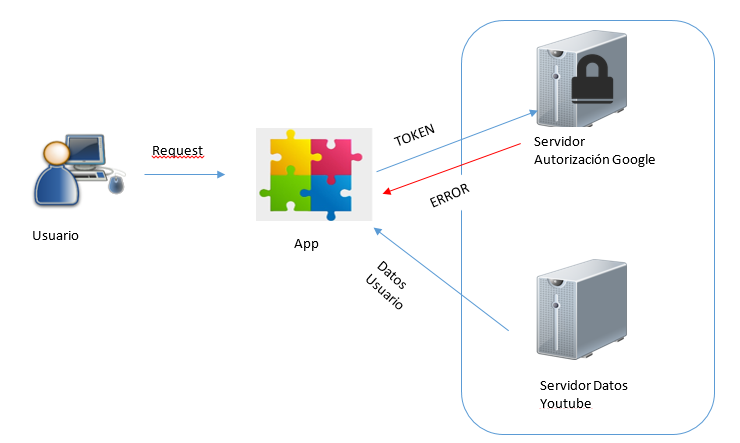
\includegraphics[width=140mm]{outh-scheme.png}
    \caption{Protocolo Oauth YouTube}
\end{figure}

\subsection{Recursos YouTube API : liveBroadcast y liveStream}

La API presenta distintos recursos, a continuación presentaremos los recursos usado para este proyecto y como a través de su manipulación podemos manejar eventos en vivo desde una aplicación.

El primero, liveBroadcast, como su propio nombre indica, se encarga de manejar la información relacionada con la emisión del evento. Este recurso tiene asociadas ciertas propiedades como la hora del evento o la privacidad, estas propiedades pueden ser definidas mediante un archivo en formato JSON, así a través de este archivo se puede configurar la emisión.



\begin{lstlisting}[language=JSON] 

{
  "kind": "youtube#liveBroadcast",
  "etag": etag,
  "id": string,
  "snippet": {
    "publishedAt": datetime,
    "channelId": string,
    "title": string,
    "description": string,
    "thumbnails": {
      (key): {
        "url": string,
        "width": unsigned integer,
        "height": unsigned integer
      }
    },
    "scheduledStartTime": datetime,
    "scheduledEndTime": datetime,
    "actualStartTime": datetime,
    "actualEndTime": datetime,
    "isDefaultBroadcast": boolean,
    "liveChatId": string
  },
  "status": {
    "lifeCycleStatus": string,
    "privacyStatus": string,
    "recordingStatus": string,
  },
  "contentDetails": {
    "boundStreamId": string,
    "boundStreamLastUpdateTimeMs": datetime,
    "monitorStream": {
      "enableMonitorStream": boolean,
      "broadcastStreamDelayMs": unsigned integer,
      "embedHtml": string
    },
    "enableEmbed": boolean,
    "enableDvr": boolean,
    "enableContentEncryption": boolean,
    "startWithSlate": boolean,
    "recordFromStart": boolean,
    "enableClosedCaptions": boolean,
    "closedCaptionsType": string,
    "projection": string,
    "enableLowLatency": boolean
  },
  "statistics": {
    "totalChatCount": unsigned long
  }
}

\end{lstlisting}

Para manipular estos datos el recurso nos proporciona varios métodos, aquí solo se explicaran algunos.

\begin{itemize}

\item \textbf{Insert}, este método crea un evento, para ello debe recibir mínimo dos  parámetros de entrada, el primero hace referencia a las partes del JSON que serán definidas(snnipet, status, contentDetails….), mientras que el segundo argumento que recibe es el propio JSON con los datos. Se deben proporcionar obligatoriamente el título, la hora de inicio y el estado de privacidad del vídeo, los demás datos si no están definidos tomarán un valor por defecto. Como respuesta a este método obtenemos el mismo JSON pero esta vez todos los campos con su valor asociado ya sea el que le hemos asignado o uno por defecto. Dentro de las propiedades obtendremos el ID del recurso que será necesario en el método BIND para poder asociarlo a un stream.

\item \textbf{List}, este método retorna una lista con todos los datos de los broadcast pedidos en función de unos parámetros de entrada. Dentro de los parámetros obligatoriamente debemos especificar las propiedades del recurso que queremos recuperar. Adicionalmente podemos aplicar ciertos filtros a los resultados.
    \begin{itemize}
        \item broadcastStatus, devuelve únicamente las emisiones que se encuentren en el estado determinado, las opciones son activo, todos, completado o sin comenzar
        \item id, es el filtro más específico devuelve únicamente el recurso asociado a un identificador
        \item maxResutls, limita los resultados obtenidos, por defecto tiene un valor de cinco pero puede tomar valores entre cero y cincuenta.
        \item broadcastType, con este filtro estipulamos que queremos obtener eventos de un tipo determinado siendo las opciones evento, una retransmisión programada a una hora determinada, persistente, un evento el cual se encuentra continuamente activo, u ambos.
    \end{itemize}
    
\item \textbf{Bind},, este método puede realizar dos acciones en función de los parámetros que reciba. Obligatoriamente debe recibir las partes del recurso, y un id perteneciente a un broadcast. Opcionalmente puede recibir un id que representa un recurso livestream, si recibe este parámetro el método enlazara ambos recursos quedando asignado a la emisión un flujo de vídeo, si por el contrario este parámetro no es proporcionado el método bind desenlazara de la emisión el flujo de vídeo si esta la tuviera.

\item \textbf{Transition} , una vez creados y enlazados ambos recursos este método nos da la posibilidad de cambiar el estado de la emisión es decir podemos hacer pública la emisión, pasar a estado de test o dar por finalizada la emisión. Para ellos deberemos proporcionarle el estado el cual queremos dar a nuestra emisión, el id de dicha emisión y las partes del recurso que queremos obtener en la respuesta.

\end{itemize}


El segundo recurso que nos encontramos es liveStream que nos permite configurar las propiedades de la ingestión del vídeo.Los métodos de este recurso son similares a los métodos del liveBroadcast con la diferencia de que son asociados a un stream y sus propiedades se definen mediante un JSON que se puede ver a continuación.

\begin{lstlisting}[language = JSON]

{
  "kind": "youtube#liveStream",
  "etag": etag,
  "id": string,
  "snippet": {
    "publishedAt": datetime,
    "channelId": string,
    "title": string,
    "description": string,
    "isDefaultStream": boolean
  },
  "cdn": {
    "format": string,
    "ingestionType": string,
    "ingestionInfo": {
      "streamName": string,
      "ingestionAddress": string,
      "backupIngestionAddress": string
    },
    "resolution": string,
    "frameRate": string
    "status": {
    "streamStatus": string,
    "healthStatus": {
      "status": string,
      "lastUpdateTimeSeconds": unsigned long,
      "configurationIssues": [{
          "type": string,
          "severity": string,
          "reason": string,
          "description": string
	}]}
    },
    "contentDetails": {
        "closedCaptionsIngestionUrl": string,
        "isReusable": boolean
    }
}

\end{lstlisting}

El método list es prácticamente igual al explicado para liveBroadcast a diferencia que el resultado que obtenemos del mismo es una lista de stream´s. Respecto al método insert su función es la de crear el recurso siendo las propiedades obligatorias a definir el título, el formato y el tipo de ingestión. Esta última propiedad, el tipo de ingestión,  establece el protocolo por el cual se transmite el flujo de vídeo a YouTube. En este campo YouTube nos proporciona dos protocolos distintos DASH o RTMP, en este proyecto el protocolo usado será RTMP debido a una mayor compatibilidad con ffmpeg, herramienta que codifica y transmite el flujo de vídeo al servidor de YouTube, dicha herramienta es explicada a continuación.

\section{FFmpeg}

FFmpeg es una colección de librerías de software libre capaz de decodificar, codificar , transcodificar, multiplexar , demultiplexar , filtrar y reproducir gran cantidad de archivos en múltiples formatos, también se encuentra disponible para distintos sistemas operativos como Linux, Mac OS X, Windows … para la mayoría de sus distribuciones.

FFmpeg presenta cuatro herramientas distintas, que son enumeradas a continuación.

\begin{itemize}

\item \textbf{ffmpeg}, herramienta que proporciona un rápida conversión de archivos de audio y vídeo a través de la línea de comandos.
\item \textbf{ffserver}, formado por un servidor de streaming para audio y vídeo, es capaz de soportar varios canales en vivo y streaming de archivos.
\item \textbf{ffplay}, es un reproductor multimedia simple basado en SDL (Simplec DirectMedia Layer) y las bibliotecas de ffmpeg.
\item \textbf{ffprob}, se encarga de reunir información de streams multimedia como formatos, bitrates, framerates…
\end{itemize}

En este proyecto únicamente se hará uso de ffmpeg como línea de comando ya que mediante esta herramienta podremos enviar flujo de vídeo al servidor de YouTube como se verá más adelante

Otro punto importante a la hora de hablar de FFmpeg son las librerías.

\begin{itemize}
    \item \textbf{libavutil}, constituye una biblioteca de apoyo de forma que se simplifica la programación incluyendo estructuras de datos, rutinas matemáticas, utilidades capa multimedia y otras muchas.
    \item \textbf{livavcodec}, esta librería está formada por codificadores y decodificadores de audio y vídeo.
    \item \textbf{libavformat}, es la parte encargada de multiplexación y demultiplexacion para diferentes formatos multimedia.
    \item \textbf{libavdevice}, esta librería contiene herramientas de entrada y salida para grabar y renderizar el contenido multimedia generado por frameworks como Video4Linux, Vfm o ALSA.
    \item \textbf{libavfilters}, proporciona filtros para contenido multimedia, filtros paso bajo, paso alto, compresores , bicuadrados …
    \item \textbf{livwscale}, esta librería realiza operaciones altamente optimizadas de escalado de imagen y espacio de color.
    \item \textbf{libswresample},  es capaz de hacer muestreo y conversiones de formato.
\end{itemize}

Como podemos ver FFmpeg es una herramienta muy potente y que nos proporciona diversas opciones.

\subsection{FFmpeg streaming}

FFmpeg proporciona dos caminos para realizar streaming el primero y el usado en este proyecto consiste en enviar directamente el flujo de vídeo a un servidor, Youtube en nuestro caso, y este retransmitirlo nuevamente. La otra alternativa consiste en retransmitir directamente a un usuario final incluso a través de la creación de múltiples salidas podría ser posible retransmitir hacía más de un usuario.
La herramienta ffmpeg a través de la línea de comandos nos permite enviar un flujo de vídeo al servidor de YouTube. Para esto hemos elegido el protocolo de transporte RTMP, dicho protocolo es mencionado en la introducción, este protocolo es capaz de intercambiar un flujo multimedia entre un reproductor flash y un servidor. El formato elegido para el vídeo es FLV (flash video player) ya que es el códec de vídeo usado por YouTube.  
Para la captura del flujo multimedia se ha optado por usar video4linux2 para el vídeo , consiste en  un API de captura de vídeo para Linux y es capaz de capturar la imagen de una webcam. Por otro lado para capturar el audio se ha elegido ALSA (Advanced Linux Sound Architecture) que es un controlador de sonido del núcleo de Linux.

\begin{figure}[H]
    \centering
    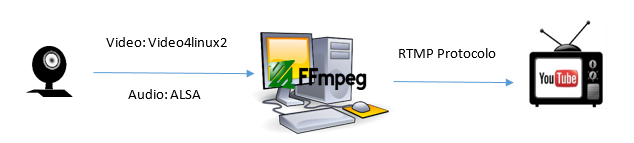
\includegraphics[width=150mm]{ffmpeg_stream.PNG}
    \caption{Esquema de retransmisión Ffmpeg}
\end{figure}

Como se podrá ver más adelante combinando todas estas herramientas que pone a nuestra disposición ffmpeg conseguiremos retransmitir un flujo de vídeo hacia YouTube.

\section{Open Broadcaster Software}

Esta aplicación conocida por sus siglas OBS, constituye un sofware libre y de código abierto para la grabación y retransmisión (streaming) de video.

OBS comenzó como un pequeño proyecto creado por Hugh "Jim" Bailey, pero creció rápidamente con la ayuda de muchos colaboradores que trabajan para mejorar la aplicación. En 2014,comenzó a desarrollarse una nueva versión conocida como OBS Multiplatform (más tarde renombrada OBS Studio) para soporte multiplataforma, siendo un programa más completo y con una API más potente.OBS Studio es un trabajo en progreso ya que, a febrero de 2016, no ha alcanzado la paridad de características con el original de la OBS, es por eso que el original aun está disponible en el sitio.

Este proyecto usa como lenguaje de programación C y C++, permite capturar fuentes de video en tiempo real, composición de escenas, codificación, grabación y retransmisión. Para la retransmisión de contenido en vivo usa RTMP como protocolo de transporte , de forma que es compatible con YouTube o Twitch entre otras plataformas.

Además la comunidad OBS ha desarrollado varios plugins que extienden sus funcionalidades como OBS remote que permite acceder remotamente a OBS a través de internet o CLR Browser Source que permite usar como fuente de vídeo un recurso web.

Este software permite realizar las mismas operaciones que ffmpeg pero de una forma mas sencilla debido a su interfaz gráfico, por lo que para usuarios menos expertos es una mejor alternativa que ffmpeg.

\begin{figure}[H]
    \centering
    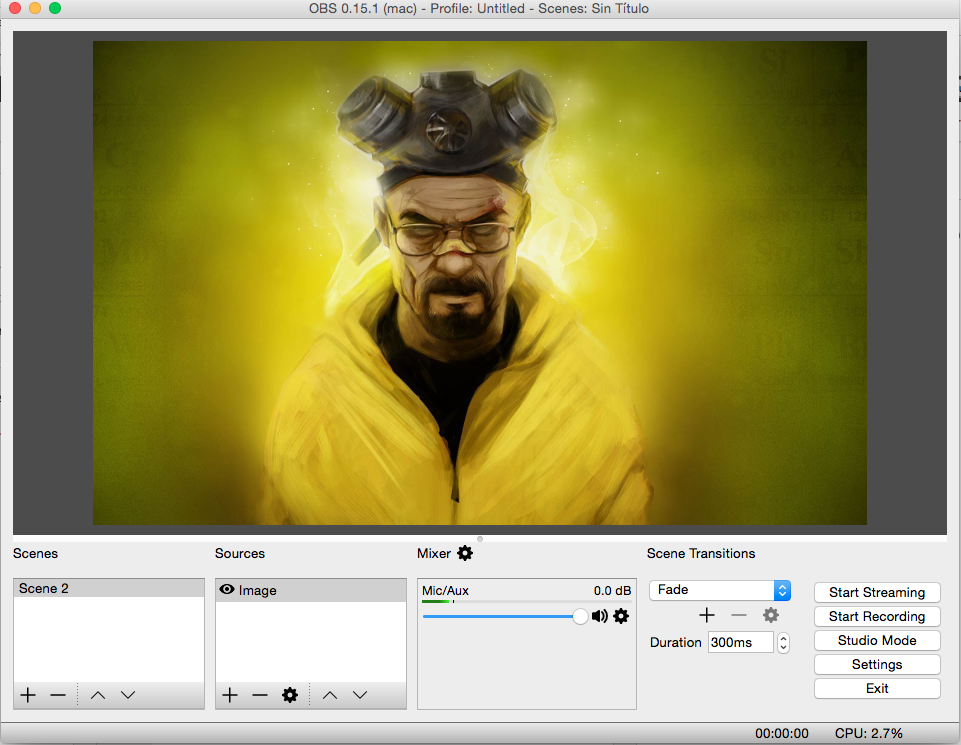
\includegraphics[width=100mm]{obs_interface.png}
    \caption{Interfaz OBS}
\end{figure}



\section{JdeRobot}

JdeRobot \footnote{http://jderobot.org}  es un entorno de desarrollo para  aplicaciones robóticas y visión por computador. Este entorno, desarrollado por el grupo de robótica de la universidad Rey Juan Carlos, simplifica el acceso a los sensores, actuadores o unidades hardware del dron. JdeRobot ha sido desarrollado en su gran mayoría usando como lenguaje de programación C++, basándose en un entorno de componentes distribuidos que pueden ser escritos en otros lenguajes como Java o Python. Finalmente estos componentes se comunican usando ICE. 

ICE hace referencia a las siglas de Internet Communications Engine y consiste en un middleware orientado a objetos desarrollado por la empresa ZeroC \footnote{https://zeroc.com} , que proporciona ayuda a la hora de desarrollar aplicaciones distribuidas ya que se encarga de todas las interacciones con los interfaces de red tales como abrir conexiones de red serializar y deserializar datos o reintentos de conexiones fallidas. Gracias a esto se puede crear conexiones entre distintas maquinas con distintos sistemas operativos o lenguajes de programación.

\begin{figure}[H]
    \centering
    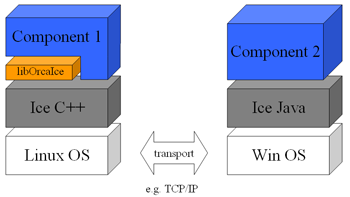
\includegraphics[width=100mm]{ice.png}
    \caption{Estructura ICE}
\end{figure}

JdeRobot también usa una distribución de ICE, llamada ICEJs  que nos da la opción de conectar navegadores usando JavaScript y los protocolos de ICE a través de websockets.

Recientemente JdeRobot ha lanzado su última versión estable JdeRobot 5.4.1. Esta versión aporta varios cambios que facilitan aún más el uso de sus herramientas. A continuación se comentan los cambios más significativos.

\begin{itemize}
    \item Cambio de SO, la nueva versión de JdeRobot es soportada únicamente por Ubuntu 16.04.
    \item Cambio en la versión de Gazebo, la versión antigua trabajaba con la versión 5 de Gazebo, con los nuevos cambios se ha pasado a usar la versión 7 de Gazebo.
    \item Actualización de la versión de ICE, este punto es importante ya que anteriormente JdeRobot trabajaba con la versión 3.5 de ICE en la cual no venía incorporado el plugin ICEJS lo que implicaba una mayor dificultad a la hora de instalar las librerías así como problemas de compatibilidad. En la nueva versión se ha pasado a usar la versión 3.6 de ICE donde si está incorporado el plugin citado.

\end{itemize}

JdeRobot ha desarrollado distintos componentes y plugins, en este proyecto se usarán dos de ellos principalmente CameraServer y un plugin desarrollado para Gazebo.

A continuación  para poder comprender completamente las tecnologías  de este proyecto vamos a hablar sobre Gazebo y su relación con JdeRobot y CameraServer.

\subsection{Gazebo}

Gazebo es un simulador 3D, que permite crear escenarios en tres dimensiones en tu ordenador con robots, obstáculos y otros muchos objetos. Gazebo fue diseñado para evaluar algoritmos y comportamientos de robots en un escenario simulado pero muy cercano a la realidad sin exponer a peligros a los robots. Para muchas aplicaciones es esencial testear las aplicaciones de forma que se pueden evitar fallos e batería, de manejo, localización o manejo entre otros. Es un proyecto de código abierto y actualmente cuenta con una gran comunidad de desarrolladores.


\begin{figure}[H]
    \centering
    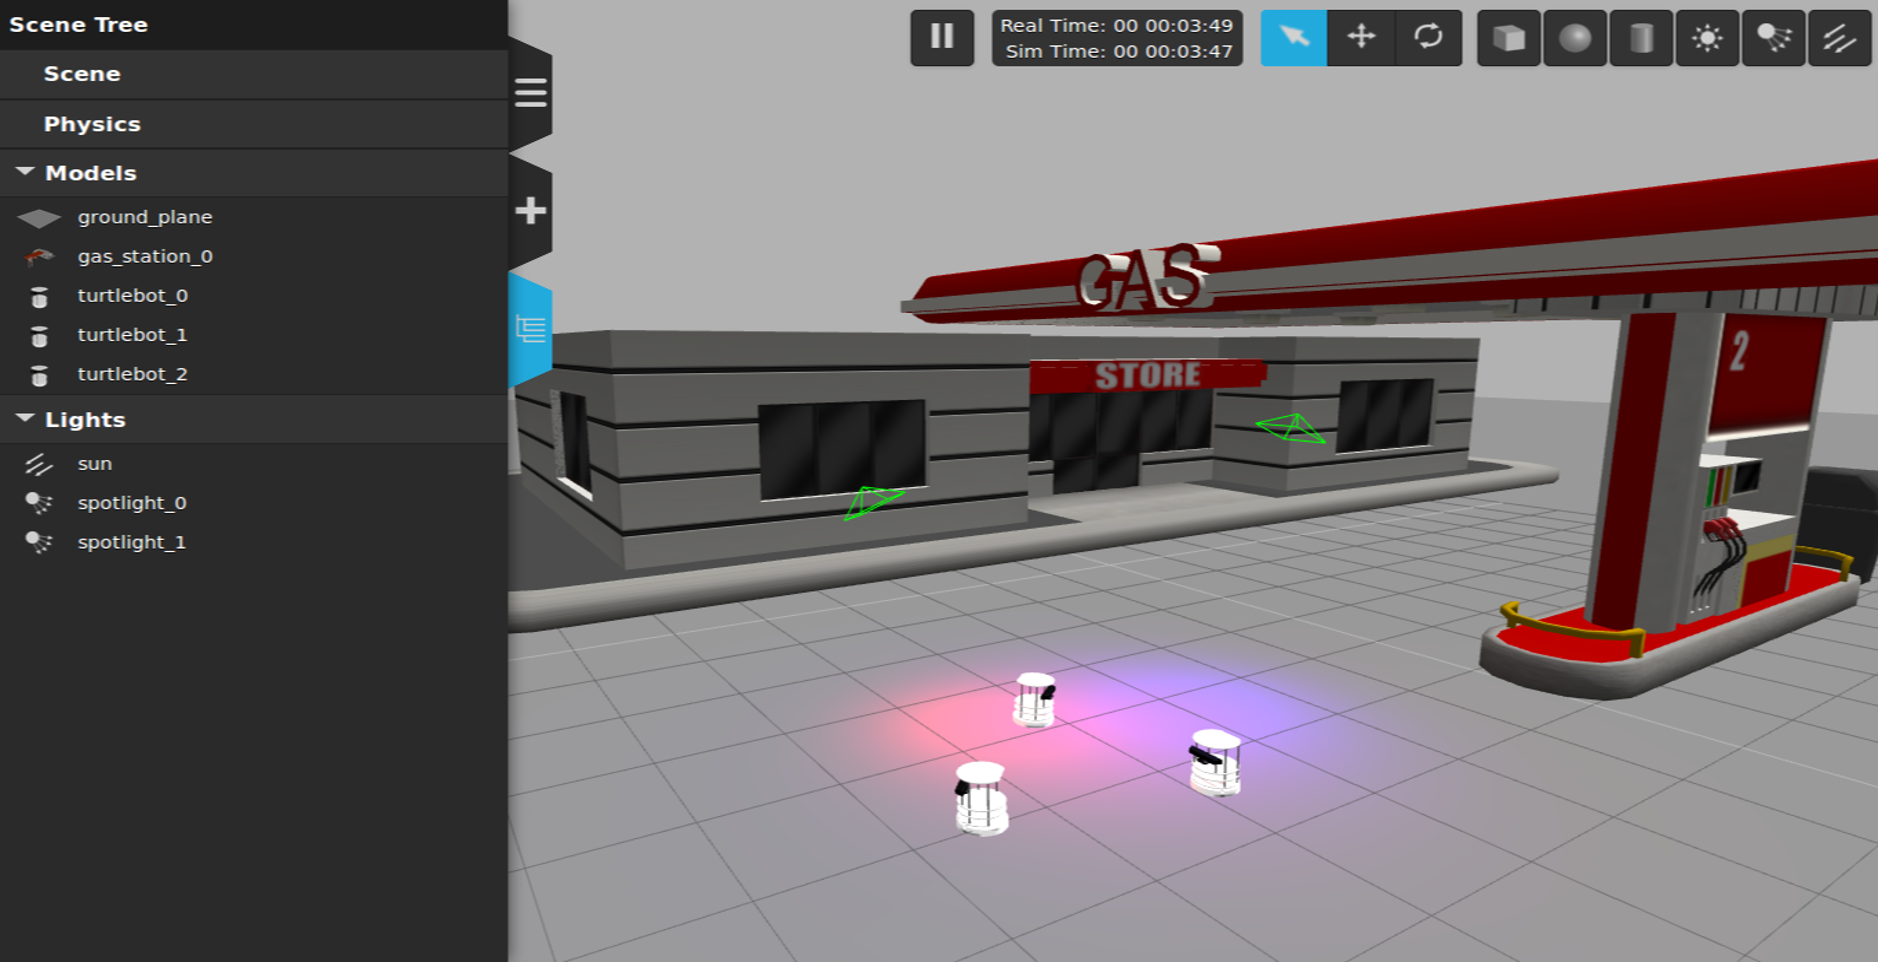
\includegraphics[width=100mm]{gazebo.png}
    \caption{Escenario creado con gazebo}
\end{figure}

JdeRobot ha desarrollado varios plugins usando Gazebo. Este plugin facilita la programación a más bajo nivel como son las conexiones de forma que podemos manejar el dron en un mundo creado por Gazebo donde podremos depurar nuestro código.


\subsection{CameraServer}

CameraServer es un componente desarrollado por JdeRobot capaz de servir N cámaras tanto reales como simuladas. Para manejar el manejo de los vídeos, internamente usa gstreamer, framework multimedia libre multiplataforma escrito en el lenguaje de programación C ,permite crear aplicaciones audiovisuales, como de vídeo, sonido, codificación.

CameraServer permite captar el vídeo de diferentes fuentes como puede ser video4linux, un archivo o un recurso web. Además es compatible Gazebo por lo que se pueden llevar a cabo simulaciones.

CameraServer proporciona una interfaz, Camera Interface, esta interfaz aporta los métodos de configuración de la cámara así como los métodos de inicio y final de la toma de imágenes. Dicho interfaz extiende otro llamado ImageProvider el cual aporta métodos de configuración de la imagen, como el formato, y métodos que recuperan imágenes. 

\begin{figure}[H]
    \centering
    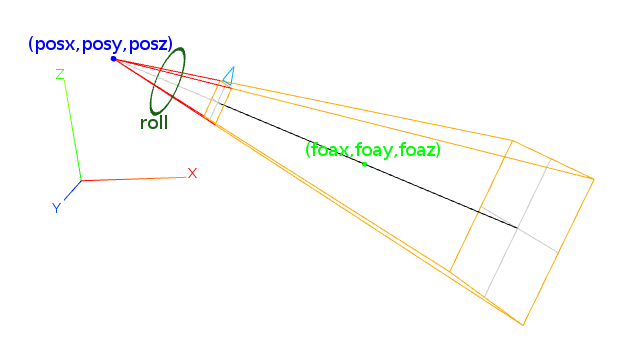
\includegraphics[width=100mm]{cameraserver.png}
    \caption{Modelo CameraServer}
\end{figure}

Se puede deducir de lo explicado anteriormente que este componente capta imágenes a una determinada velocidad para finalmente formar un vídeo.


